%!TEX TS-program = pdflatex
%!TEX encoding = UTF-8 Unicode

\documentclass[12pt,a4paper,oneside,english,italian]{book}

\usepackage[utf8]{inputenc}

\usepackage{extensions/uniudtesi}

\usepackage[nottoc]{tocbibind}
\usepackage{babel}[italian]
\usepackage{indentfirst}
\usepackage{scalerel}
\usepackage[ruled,vlined,linesnumbered]{algorithm2e}

\graphicspath{{./figure/}}
\usepackage{amsmath,amsfonts,amssymb,amsthm}
\usepackage{latexsym}
\usepackage{graphicx} % [demo] is just for the example
\usepackage{wrapfig}
\usepackage{mathabx}
\usepackage{cancel}[makeroom]

\newcommand{\N}{\mathbb{N}}
\newcommand{\Z}{\mathbb{Z}}
\newcommand{\Q}{\mathbb{Q}}
\newcommand{\R}{\mathbb{R}}
\newcommand{\C}{\mathbb{C}}

% IR functions
\newcommand{\sco}{\text{score}}
\newcommand{\tf}{\text{tf}}
\newcommand{\tfp}{\text{tf}_p}
\newcommand{\idf}{\text{idf}}
\newcommand{\rc}{\text{rc}}
\newcommand{\rel}{\text{rel}}
\newcommand{\re}{\text{Re}}
\newcommand{\preci}{\text{Pre}}


\DeclareMathOperator{\traccia}{tr}
\DeclareMathOperator{\sen}{sen}
\DeclareMathOperator{\arcsen}{arcsen}
\DeclareMathOperator*{\maxlim}{max\,lim}
\DeclareMathOperator*{\minlim}{min\,lim}
\DeclareMathOperator*{\deepinf}{\phantom{\makebox[0pt]{p}}inf}

\newcommand{\varsum}[3]{\sum_{#2}^{#3}\!
   {\vphantom{\sum}}_{#1}\;}
\newcommand{\varprod}[3]{\sum_{#2}^{#3}\!
   {\vphantom{\sum}}_{#1}\;}
\newcommand*{\tokenbox}[1]{\framebox{#1}}

%%%%%%%%%%%%%%%%%%%%%%%%%%%%%%%%%%%%%%%%%%%%%%%%%%%%%%%%%%%

\theoremstyle{plain}
\newtheorem{teorema}{Teorema}[chapter]
\newtheorem{proposizione}[teorema]{Proposizione}
\newtheorem{lemma}[teorema]{Lemma}
\newtheorem{corollario}[teorema]{Corollario}

\theoremstyle{definition}
\newtheorem{definizione}[teorema]{Definizione}
\newtheorem{esempio}[teorema]{Esempio}
\newtheorem{problema}[teorema]{Problema}

\theoremstyle{remark}
\newtheorem{osservazione}[teorema]{Osservazione}

\newcommand{\fsamp}{\textsc{F-samp}\xspace}
\newcommand{\base}{\textsc{base}\xspace}
\newcommand{\fcount}{\textsc{F-count}\xspace}


\usepackage{makeidx}
\makeindex

% Ridefiniamo la riga di testa delle pagine:
\usepackage{fancyhdr}
\pagestyle{fancy}
\renewcommand{\chaptermark}[1]{\markboth{#1}{}}
\renewcommand{\sectionmark}[1]{\markright{\thesection\ #1}}
\fancyhf{}
\fancyhead[LE,RO]{\bfseries\thepage}
\fancyhead[LO]{\bfseries\rightmark}
\fancyhead[RE]{\bfseries\leftmark}
\renewcommand{\headrulewidth}{0.5pt}
\renewcommand{\footrulewidth}{0pt}
\setlength{\headheight}{14.5pt}

  \titoloeng{Exploring BM25P\cr hyperparameters space}
  \titolo{Esplorazione dello spazio degli iperparametri di BM25P}
  \laureando{Federico Silvestri}
  \annoaccademico{2019-2020}
  %\facolta{Scienze Matematiche, Fisiche e Naturali}
  \corsodilaureatriennalein{Informatica}
  \relatore[Prof.]{Maria Simi}
  \relatoreDue[Dott.]{Cristina Ioana Muntean}
  \dedica{Dedicato alle persone più care \\ che ho conosciuto e che tuttora, anche se in modo diverso, \\ sono con me. }

% Per l'ipertesto:
 \usepackage{hyperref} % gia' caricato da uniudtesi
 \hypersetup{
  bookmarksopen, % default
  bookmarksopenlevel=2, % default;
  pdftitle={Exploring BM25P hyperparameter space},
  pdfauthor={Federico Silvestri},
  pdfsubject={Thesis of Bachelor Degree in Computer Science},
  pdfkeywords={Thesis Bachelor Degree Computer Science Federico Silvestri}
  }
  
\usepackage{listings}
\usepackage{xcolor}
\definecolor{listinggray}{gray}{0.9}
\definecolor{lbcolor}{rgb}{0.9,0.9,0.9}
\lstset{
	backgroundcolor=\color{lbcolor},
	tabsize=2,    
	language=Java,
	basicstyle=\scriptsize,
	upquote=true,
	aboveskip={1.5\baselineskip},
	columns=fixed,
	showstringspaces=false,
	extendedchars=false,
	breaklines=true,
	prebreak = \raisebox{0ex}[0ex][0ex]{\ensuremath{\hookleftarrow}},
	frame=single,
	numbers=left,
	showtabs=false,
	showspaces=false,
	showstringspaces=false,
	identifierstyle=\ttfamily,
	keywordstyle=\color[rgb]{0,0,1},
	commentstyle=\color[rgb]{0.026,0.112,0.095},
	stringstyle=\color[rgb]{0.627,0.126,0.941},
	numberstyle=\color[rgb]{0.205, 0.142, 0.73},
}

 \lstset{
 	backgroundcolor=\color{lbcolor},
 	tabsize=2,
 	language=Java,
 	captionpos=b,
 	tabsize=2,
 	frame=lines,
 	numbers=left,
 	numberstyle=\tiny,
 	numbersep=5pt,
 	breaklines=true,
 	showstringspaces=false,
 	basicstyle=\footnotesize,
 	% identifierstyle=\color{magenta},
 	keywordstyle=\color[rgb]{0,0,1},
 	commentstyle=\color[rgb]{0,0.39,0},
 	stringstyle=\color{red},
 	morecomment=[l][\color{magenta}]{\#}
 }


\usepackage{bold-extra}
\usepackage{lmodern}

\begin{document}
\nocite{*}
\renewcommand{\theequation}{\thechapter.\arabic{equation}}
\renewcommand{\thesection}{\thechapter.\arabic{section}}

\frontmatter

\maketitle

\cleardoublepage

\tableofcontents

% \listoffigures

\mainmatter

% \let\cleardoublepage\clearpage
 
 \chapter{Descrizione del tirocinio}

Il tirocinio si è svolto quasi sempre in modalità telematica,
sia perché la situazione dovuta al COVID-19 non ha concesso
gli spostamenti, sia perché  il lavoro che doveva essere svolto
era per lo più individuale.
Sono stato supervisionato principalmente da tre persone,
le quali mi hanno dato degli obiettivi da raggiungere per ogni
step del tirocinio,
fino ad arrivare alla conclusione.
Il codice implementato risiede in piccola
quantità nell'appendice di questa relazione,
e invece tutto il progetto e tutte le sperimentazioni
sono disponibili sulla pagina personale di \href{https://github.com/federicosilvestri/bm25p-thesis}{GitHub}.

Il tirocinio si è concluso una volta raggiunti i risultati
previsti, e le ore totali impiegate sono state circa 320.

\subsection{Basi di partenza}
Questo tipo di tirocinio si è basato
sullo studio di una materia non trattata nel corso di laurea triennale:
\textit{Information Retrieval} (\textit{IR}).
Tale materia è risultata abbastanza facile da comprendere grazie
al materiale fornito dai tutor e alla loro disponibilità.
Una volta approfondito lo studio è iniziata la fase sperimentale,
cioè la progettazione e implementazione di svariati meccanismi per la ricerca 
degli iperparametri ottimi di BM25P.

L'algoritmo BM25P è un'estensione della funzione di ranking
di BM25, un noto algoritmo nel ramo dell'\textit{IR}.
BM25P è stato ideato e pubblicato su ACM dal C.N.R.
stesso nel 2019.\cite{10.1145/3331184.3331373}

Per concludere si sono verificate alcune ipotesi
che erano state fatte dai tutor come premessa
del tirocinio stesso.

\subsection{Linguaggi utilizzati}
Devo scriverli meglio: Java, bash, Python, niente di più

 
\chapter{Introduzione}
Al giorno d'oggi cercare informazioni sul web è diventata una delle operazioni più comuni e più richieste:
utilizzare lo smartphone per eseguire una ricerca sui punti di interesse di una città, o per scoprire la ricetta di un dolce è capitato quasi a tutte le persone.
Le statistiche elaborate direttamente da Google affermano che ogni secondo vengono richieste circa \textit{40.000} query, per un totale
giornaliero di \textit{3,5 miliardi}.
Siamo arrivati persino a parlare di memoria \textit{transattiva}, ovvero di una memoria condivisa tra tutti gli utenti e disponibile attraverso il web.
Ogni essere umano che possiede un qualunque mezzo tecnologico è in grado di accedervi in svariati modi, per esempio facendo una ricerca tramite Siri, Google oppure Alexa.
Tale memoria non consiste nel memorizzare l'informazione stessa, ma in come giungere ad essa.

Non è solo all'interno del web che c'è la necessità di un sistema di ricerca. Si pensi per esempio a Spotlight di Mac OS che
viene utilizzato per reperire informazioni da file di testo, audio, immagini e anche news dalla rete.

Il ruolo dell'Information Retrieval al giorno d'oggi è dunque di fondamentale importanza.
Per questo c'è stata la necessità di sviluppare gli algoritmi in tutte le dimensioni, a partire dall'architettura delle macchine sulle quali i documenti vengono archiviati a come i documenti stessi vengono strutturati.

In questa tesi di tirocinio verrà illustrato \textit{Terrier}: una piattaforma sviluppata dall'università di Glasgow
per sperimentare gli algoritmi legati all'Information Retrieval, anche su collezioni di dati nell'ordine dei terabyte.  Successivamente il focus si sposterà
sugli algoritmi di ranking, dei quali sarà utilizzato BM25P, una versione di BM25 migliorata dal gruppo ISTI del CNR di Pisa.
Verranno illustrati una serie di algoritmi il cui scopo è quello di ricercare, all'interno di uno spazio multidimensionale,
gli \textit{iperparametri} di BM25P, incrementando dunque le prestazioni rispetto a BM25 stesso.

Attraverso dei test statistici si dimostrerà infine che i due modelli di ranking sono decisamente diversi ed è possibile
inferire in quali parti (\textit{passages}) del documento sono contenute le informazioni più \textit{rilevanti}
e questo varierà in base al tipo di collezione di testi.

\section{Architettura generale}
In questo capitolo verrà illustrata l'architettura generale di un sistema di IR (\textit{Information Retrieval}) e verranno
descritti alcuni processi che sono stati oggetto di studio del tirocinio.

Quando si parla di sistema di IR, oppure in termini più quotidiani di motore di ricerca,
siamo spesso abituati a vederlo come un meccanismo di interrogazione dove l'utente
digita come input un testo, chiamato query e il motore risponde con una serie di risultati. Tali risultati
sono visualizzati dall'utente come una lista di documenti che contengono informazioni
rilevanti secondo la query.
\`E immediato pensare all'esempio di Google, dove il fruitore digita una serie di termini
all'interno del  form e dopo qualche secondo gli vengono restituiti tutti i link a pagine web, che
sono in qualche modo collegate a ciò che l'utente stava realmente cercando.
Quello che sta dietro a tutto questo processo, che sembra essere quasi immediato nell'esempio di Google, è
in realtà un lavoro molto complesso e richiede molto tempo.
La fase in cui l'utente è abituato ad essere partecipe è quella finale, ovvero
il \textit{recupero}; ma prima di poter parlare di ciò è necessario illustrare la fase primaria, l'\textit{indicizzazione}.

\paragraph{Alcune definizioni}
Per essere più chiari, conveniamo alcune definizioni di termini tecnici che in altri contesti possono essere attribuiti
a concetti diversi.

\begin{definizione}\label{def:token}
	Un token è un'istanza di una sequenza di caratteri, in un documento $d \in \mathcal{D}$, che
	sono raggruppati tra di loro come un'unità semanticamente utile.
\end{definizione}

\begin{esempio}[tokenizzazione]
	Nella frase "Nulla si crea, nulla si distrugge ma tutto si trasforma" i token sono i seguenti:
	\tokenbox{nulla} \tokenbox{si} \tokenbox{crea} \tokenbox{nulla} \tokenbox{si} \tokenbox{distrugge}
	\tokenbox{ma} \tokenbox{tutto} \tokenbox{si} \tokenbox{trasforma}.
\end{esempio}

Un altro concetto importante è quello di \textit{tipo}.

\begin{definizione}[tipo]\label{def:tipo}
	Un tipo è una classe di token con la solita sequenza di caratteri.
\end{definizione}
\begin{esempio}
	Consideriamo la frase dell'esempio precedente. I tipi sono 7, mentre i token sono 10. Abbiamo dunque
	3 token che si ripetono.
\end{esempio}
\begin{definizione}[query]\label{def:query}
	Una query è un multinsieme di token, che rappresenta l'input che il motore di ricerca
	riceve dall'utente. 
\end{definizione}

\begin{esempio}
	Se si volessero cercare dei manuali tecnici sul linguaggio Python, si potrebbe esprimere 
	tale necessità attraverso la query $q$: \tokenbox{manuali} \tokenbox{python}.
	\\
	\\
	Un altro esempio potrebbe essere quello di voler ricercare i componenti
	elettronici inventati nel 1950. La query potrebbe essere $q$ : \tokenbox{componenti}
	\tokenbox{elettronici} \tokenbox{1950}.
\end{esempio}

Da notare che il concetto di multinsieme deriva dal fatto che si vuole tenere traccia in modo esplicito 
della molteplicità dei token nella query stessa.

\paragraph{Fase di indicizzazione}
Per poter offrire quella velocità che si richiede durante la fase di \textit{recupero} è necessario: aver ``preparato"
una struttura dati che sia completa, ovvero che comprenda tutte le informazioni necessarie e 
rapida da scorrere, cioè che le informazioni che si stanno cercando devono poter essere recuperate
il prima possibile.  Un esempio abbastanza esplicativo è quello dell'addetto alla biblioteca che deve rispondere
alle richieste degli studenti. Se egli non conoscesse i libri che sono parte della biblioteca, per ogni richiesta
dovrebbe scorrere tutta la lista e capire se quel dato libro può essere utile oppure no.
Questo esempio rappresenta il fatto che l'addetto non è in possesso di una struttura in grado
di accedere solo alle informazioni necessarie ed è dunque inefficiente.
Se quindi non ci fosse un indice, per un motore di ricerca sarebbe troppo dispendioso elaborare tutti
i documenti ``su richiesta".
La fase di \textit{indexing} ha lo scopo di costruire una struttura dati, chiamata indice, che consenta
di velocizzare la fase successiva, il \textit{recupero}.

Dal punto di vista delle prestazioni tale fase è quella con il  dispendio computazionale
più elevato, sia in termini di spazio che di tempo.
Questo perché si devono analizzare tutti i documenti della collezione ed eseguire una serie di elaborazioni
su di essi.

Il seguente algoritmo illustra in modo abbastanza basico ma intuitivo, la funzione eseguita dall'indexer.
\begin{algorithm}[h]
	\small
	\DontPrintSemicolon
	\SetKwInOut{Input}{Input}
	\SetKwInOut{Output}{Output}
	\Input{$\mathcal{D} $ collezione di documenti}
	\Output{$\mathcal{I}$ indice}
	\BlankLine
	$\mathcal{I} = generateEmptyIndex()$\;
	\ForEach{$d \in \mathcal{D}$}{
		$tokenizer = getTokenizer(d)$\;
		\While{$token = tokenizer.nextToken()$}{
			$n = normalizeToken(token)$\;
			$updateIndex(\mathcal{I}, n, d)$\;
		}
	}
	\Return{$\mathcal{I}$}
	\caption{\textsc{}}
	\label{alg:indexing}
\end{algorithm}
L'idea alla base è quella di rappresentare un documento come un flusso di token, il che è sempre possibile
poiché conveniamo che in questo campo dell'IR i documenti sono solo di tipo testuale.
Il token prima di essere passato alla funzione $updateIndex$ viene normalizzato. La normalizzazione è un processo
che si occupa di risolvere alcuni problemi legati al riconoscimento di  quando due token sintatticamente diversi
hanno invece la solita semantica.\footnote{Potrebbe essere necessario uno step in più per risolvere il problema della codifica, poiché alcune lingue posseggono caratteri che non tutte le codifiche hanno. Per esempio le lingue cirillica e cinese.}

Tale processo può essere schematizzato nel seguente modo, dove a sinistra viene indicato
il nome della normalizzazione e a destra una breve descrizione.

\begin{itemize}
	\item[\textbf{Casing:}] le lettere maiuscole vengono convertite in minuscole oppure viceversa, in base al tipo di convenzione utilizzata.
	\item[\textbf{Accenti:}] le parole con accenti vengono convertite in parole senza accenti.
	\item[\textbf{Lemmatizzazione:}] vengono convertite le forme flesse delle parole in una forma canonica, cioè nel lemma.
\end{itemize}

\begin{esempio}[normalizzazione]
	Sia data la seguente frase: ``\textit{Mi piacciono tutte le auto che sono elettriche}".
	Utilizzando le tecniche elencate in precedenza, i token normalizzati risultano:
	\tokenbox{Mi} \tokenbox{piacere} \tokenbox{tutte} \tokenbox{le} \tokenbox{auto}
	\tokenbox{che} \tokenbox{essere} \tokenbox{elettriche}.
\end{esempio}

\subparagraph{Indice invertito}
Una volta che il token è stato normalizzato si procede all'aggiornamento dell'indice, ovvero alla costruzione (o aggiornamento)
dell'indice invertito. Tale struttura è definita come una lista di coppie
$\langle token, postingList \rangle$ dove \textit{postingList} è una lista di \textit{identificatori di documenti}.
In questo modo possiamo capire il token $x$ in quali documenti è contenuto, cercando dentro l'indice
invertito la posizione di $x$ e accedendo alla sua \textit{postingList}.

\begin{figure}[h]
	\label{fig:invertedIndex}
	\centering
	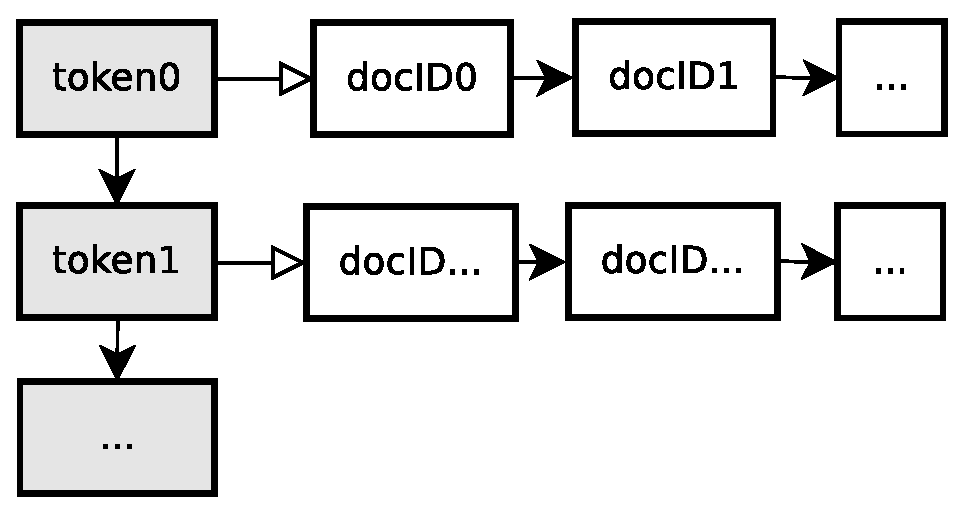
\includegraphics[scale=0.4]{InvertedIndex.eps}
\end{figure}

\pagebreak

Ritornando all'esempio della biblioteca, se l'addetto avesse a disposizione l'indice invertito potrebbe:
\begin{enumerate}
	\item raccogliere la query $\mathcal{Q}$ dello studente
	\item normalizzare $\mathcal{Q}$
	\item $\forall t.t\in Q$ cercare all'interno dell'indice invertito il termine $t$ e \textit{ritornare} la \textit{postingList} associata
\end{enumerate}

In questo modo tutti i documenti che contengono almeno una volta un termine della query verrebbero mostrati
agli studenti, ma ovviamente non tutti possono essere rilevanti per la ricerca. Il problema dunque si è ridotto
a come utilizzare l'indice invertito per capire quanto la query sia associata al documento in questione ed è per questo
motivo che viene introdotta la fase di \textit{recupero}.

\paragraph{Fase di recupero}
Lo scopo della fase di \textit{recupero} è quello di utilizzare l'indice invertito e affinare il modo con cui
i documenti vengono proposti all'utente. Tali documenti sono comunemente chiamati \textit{risultati}.
Il processo prende anche il nome di \textit{ranking}, poiché l'idea alla base è quella di attribuire
un punteggio ad ogni risultato e costruire una lista ordinata in senso crescente.
Ovviamente il primo risultato è quello per il quale il sistema di ranking attribuisce
il  punteggio più alto e dunque il risultato è rilevante per la query $q$. 
Tale processo viene fatto ogni volta che l'utente
interroga il sistema, per cui deve essere veloce, efficiente ed efficace.

L'articolo \cite{10.1016/j.ipm.2016.05.004} mostra una serie di tecniche che possono essere
utilizzate per valutare il compromesso tra qualità di un ranker ed efficienza, 
alcune delle quali sono state utilizzate nell'ambito di questo tirocinio.\\
Per essere più precisi possibile, possiamo definire la funzione di \textit{scoring} nel seguente modo:

\begin{definizione}\label{def:funzione_di_score_ideale}
	Una funzione di scoring ideale $f(d,q) : \mathcal{D} \times \mathcal{Q} \rightarrow \mathbb{R}$ è tale
	se e solo se
	$$
	f(d_1,q_1) \geq f(d_2, q_2) \implies \rel(d_1, q_1) \geq \rel(d_2, q_2)
	$$
dove $\rel(d,q)$ è la rilevanza del documento $d$ per la query $q$, calcolata a priori.	
\end{definizione}

Tale definizione delinea una funzione di scoring ideale, per la quale non esiste un algoritmo che
la calcoli. Possiamo però accontentarci di funzioni che la approssimino, facendo uso di euristiche basate sulla statistica.

Lo scopo di $f$ può esser visto anche come quello di produrre un elenco ordinato il più possibile uguale a quello
che produrrebbe la funzione $\rel$. Ciò comporta che anche se i valori di $f$ fossero scalati rispetto a quelli di $\rel$,
$f$ rappresenterebbe comunque una buona approssimazione.

\begin{esempio}
	Sia $\mathcal{L}= \left\{d_1, d_3, d_5, d_6, d_8 \right\}$ l'elenco ordinato prodotto
	dalla funzione ideale di scoring secondo una query $q$. Applicando $\rel$ ad esso si ottiene dunque la seguente catena
	di disuguaglianze: \footnote{La funzione $\rel$, nell'esempio in questione, non è stata provvista del parametro $q$ per semplicità di trattazione.}
	
	$$
	\rel(d_1) \geq \rel(d_3) \geq \rel(d_5) \geq \rel(d_6) \geq  \rel(d_8)
	$$
	
	\`E possibile trovare adesso una funzione che assuma valori diversi da $\rel$, ma che produca il solito ordine,
	ad esempio:
	
	\begin{align*}
	\rel(\mathcal{L}) = \left\{1, 1, 1, 0, 0\right\} \\
	f(\mathcal{L}) = \left\{8, 8, 7, 3, 1\right\}
	\end{align*}
	
\end{esempio}

\pagebreak

Nei prossimi capitoli verranno descritte le funzioni di scoring che propongono BM25 e BM25P, le quali si basano sul concetto di \textit{Term Frequency} e \textit{Inverse Document Frequency}.
Prima di concludere la visione generale diamo la definizione di alcuni concetti che sono utilizzati durante il \textit{recupero}.

\begin{definizione}[Raw Count]\label{def:raw_count}
	$\rc(q, d) : \mathcal{Q} \times \mathcal{D} \rightarrow \mathbb{N}$ è detto raw count, cioè il numero di volte che
	il termine $q$ occorre nel documento $d$.
\end{definizione}

\begin{definizione}[Term Frequency]\label{def:}
	La funzione $\tf(q,d)$, acronimo di Term Frequency, è una funzione che calcola la frequenza del
	termine $q \in \mathcal{Q}$ nel documento $d \in \mathcal{D}$.
	Tale valore si discosta da quello di $\rc$, poiché solitamente è normalizzato o in scala logaritmica
	oppure in base alla lunghezza del documento.
	
	\begin{itemize}
		\item $\tf(q,d) = \log_{k}(1+\rc(q,d))$ con $k>1$
		\item $\tf(q,d) = \frac{rc(q,d)}{|d|}$ dove $|d|$ è il numero totale di token nel documento
	\end{itemize}
\end{definizione}

\begin{definizione}[Inverse Document Frequency]\label{def:idf}
	$$
	\idf(q, \mathcal{D}) = \log_{k>1}{
		\frac{\#\mathcal{D}}{
			\#
			\left\{
			d \in \mathcal{D} \middle \lvert \rc(q,d) > 0
			\right\} 
		}
	}
	$$
	
	Tale misura esprime quanta informazione una parola, o più un generale un token, fornisce.
	Può essere anche vista come la misura della rarità, cioè quanto è comune il termine $q$
	nella collezione di documenti $\mathcal{D}$.
\end{definizione}





 
\section{Architettura generale}
In questo capitolo verrà illustrata l'architettura generale di un sistema di IR e verranno
descritti alcuni processi che sono stati oggetto di studio del tirocinio.
Quando si parla di sistema di IR, oppure in termini più quotidiani di \textit{search engine},
siamo spesso abituati a vederlo come un sistema di interrogazione dove l'utente
digita come input un testo, chiamato query e il motore risponde con una serie di risultati. Tali risultati
sono visualizzati all'utente come una lista di documenti che contengono informazioni
rilevanti secondo la query.
\`E immediato pensare all'esempio di Google, dove l'utente digita una serie di termini
all'interno del  form e dopo qualche secondo gli vengono restituiti tutti i link a pagine web che
sono in qualche modo collegate a ciò che l'utente stava realmente cercando.
Quello che sta dietro a tutto questo processo, che sembra essere quasi immediato nell'esempio di Google, è
in realtà un lavoro molto complesso e lungo.
La fase che l'utente è abituato ad esserne partecipe è la fase finale, ovvero
il \textit{Retrieving}. Ma prima di poter parlare di ciò è necessario illustrare la fase primaria, l'\textit{Indexing}.

\paragraph{Alcune definizioni}
Per essere più chiari, conveniamo alcune definizioni di termini tecnici che al giorno d'oggi possono essere attribuiti
a concetti diversi.

\begin{definizione}\label{def:token}
	Un token è un'istanza di una sequenza di caratteri, in un documento $d \in \mathcal{D}$, che
	sono raggruppati tra di loro come un'unità semanticalmente utile.
\end{definizione}

\begin{esempio}[tokenizzazione]
	Nella frase "Nulla si crea, nulla si distrugge ma tutto si trasforma" i token sono i seguenti:
	\tokenbox{nulla} \tokenbox{si} \tokenbox{crea} \tokenbox{nulla} \tokenbox{si} \tokenbox{distrugge}
	\tokenbox{ma} \tokenbox{tutto} \tokenbox{si} \tokenbox{trasforma}.
\end{esempio}

Un altro concetto importante è il concetto di tipo.
\begin{definizione}[tipo]\label{def:tipo}
	Un tipo è una classe di token con la solita sequenza di caratteri.
\end{definizione}
\begin{esempio}
	Consideriamo la frase dell'esempio precedente. I tipi sono 7, mentre i token sono 10. Abbiamo dunque
	3 token che si ripetono.
\end{esempio}
\begin{definizione}[query]\label{def:query}
	Una query è un multinsieme di token, che rappresenta l'input che il motore di ricerca
	riceve dall'utente. 
\end{definizione}
Da notare che il concetto di multinsieme deriva dal fatto che si vuole tenere traccia in modo esplicito 
della molteplicità
dei termini nella query stessa.

\begin{definizione}[termine]\label{def:temine}
	Un termine è un tipo di una query.
\end{definizione}

\paragraph{Fase di indexing}
Per poter offrire quella velocità che si richiede durante la fase di retrieving è necessario aver ``preparato"
una struttura dati che sia completa, ovvero che comprenda tutte le informazioni necessarie, e 
rapida da scorrere, ovvero che le informazioni che si stanno cercando devono poter essere recuperate
il prima possibile.  Un esempio abbastanza esplicativo è quello dell'addetto alla biblioteca che deve rispondere
alle richieste degli studenti. Se l'addetto non conoscesse i libri che sono parte della biblioteca, per ogni richiesta
dovrebbe scorrere tutta la lista e capire se quel dato libro può essere utile oppure no.
Questo esempio rappresenta il fatto che l'addetto non è in possesso di una struttura in grado
di accedere solo alle informazioni necessarie ed è dunque inefficiente.
Se quindi non ci fosse un indice, per un motore di ricerca sarebbe troppo dispendioso elaborare tutti
i documenti "su richiesta".
La fase di indexing ha lo scopo di costruire una struttura dati, chiamata indice, che consenta
di velocizzare la fase successiva, il Retrieving.
Dal punto di vista delle prestazioni tale fase è quella con il  dispendio computazionale
più elevato, sia in termini di spazio che di tempo.
Questo perché si devono analizzare tutti i documenti della collezione ed eseguire una serie di elaborazioni
su di essi.
Il seguente algoritmo illustra in modo abbastanza basico ma intuitivo, la funzione eseguita dall'indexer.
\begin{algorithm}[h]
	\small
	\DontPrintSemicolon
	\SetKwInOut{Input}{Input}
	\SetKwInOut{Output}{Output}
	\Input{$\mathcal{D} $ collezione di documenti}
	\Output{$\mathcal{I}$ indice}
	\BlankLine
	$\mathcal{I} = generateEmptyIndex()$\;
	\ForEach{$d \in \mathcal{D}$}{
		$tokenizer = getTokenizer(d)$\;
		\While{$token = tokenizer.nextToken()$}{
			$n = normalizeToken(token)$\;
			$updateIndex(\mathcal{I}, n, d)$\;
		}
	}
	\Return{$\mathcal{I}$}
	\caption{\textsc{}}
	\label{alg:indexing}
\end{algorithm}
L'idea alla base è quella di rappresentare un documento come un flusso di token, il che è sempre possibile
poiché conveniamo che in questo campo di information retrieval i documenti sono solo di tipo testuale.
Il token prima di essere passato alla funzione $updateIndex$ viene normalizzato. La normalizzazione è un processo
che si occupa di risolvere alcuni problemi legati al riconoscere quando due token sintanticamente diversi
hanno invece la solita semantica\footnote{Potrebbe essere necessario uno step in più per risolvere il problema della codifica, poiché alcune lingue posseggono caratteri che non tutte le codifiche hanno. Per esempio le
lingue cirillica e cinese.}
Tale processo può essere schematizzato nel seguente modo, dove a sinistra viene indicato
il nome della normalizzazione e a destra una breve descrizione.
\begin{itemize}
	\item[Casing] le lettere maiuscole vengono convertite in minuscole
	\item[Accenti] le parole con accenti vengono convertite in parole senza accenti
	\item[Stemming] i verbi vengono convertiti in una forma normale, per esempio nel tempo infinito.
	\item[Lemmization] le parole plurali vengono convertite in singolari
\end{itemize}

\begin{esempio}[normalization]
	Sia data la seguente frase: ``\textit{Mi piacciono tutte le auto che sono elettriche}".
	Utilizzando le tecniche elencate in precedenza, i token normalizzati risultano:
	\tokenbox{Mi} \tokenbox{piacere} \tokenbox{tutte} \tokenbox{le} \tokenbox{auto}
	\tokenbox{che} \tokenbox{essere} \tokenbox{elettriche}.
\end{esempio}

\subparagraph{Indice invertito}
Una volta normalizzato si procede all'aggiornamento dell'indice, ovvero alla costruzione (o aggiornamento)
dell'indice invertito. Tale struttura è definita come una lista di coppie
$\langle token, PostingList \rangle$ dove PostingList è una lista di \textit{identificatori di documenti}.
In questo modo possiamo sapere il token $x$ in quali documenti è contenuto, cercando dentro l'indice
invertito la posizione di $x$ e accedendo alla sua \textit{postingList}.

\begin{figure}[h]
	\label{fig:invertedIndex}
	\centering
	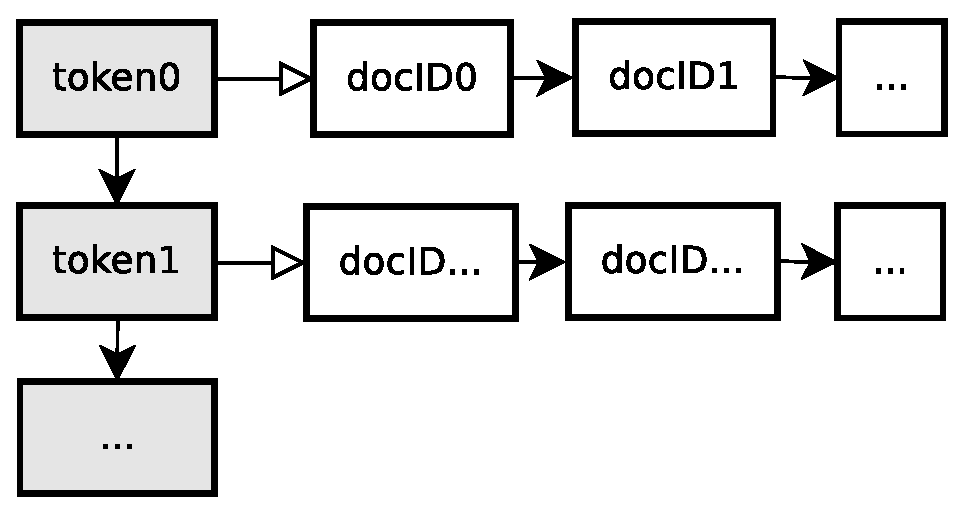
\includegraphics[scale=0.4]{InvertedIndex.eps}
\end{figure}

Ritornando all'esempio della biblioteca, se l'addetto avesse a disposizione l'indice invertito potrebbe:
\begin{enumerate}
	\item Raccogliere la query $\mathcal{Q}$ dello studente
	\item Normalizzare $\mathcal{Q}$
	\item $\forall t.t\in Q$ cercare all'interno dell'indice invertito il termine $t$ e \textit{ritornare} la \textit{postingList} associata
\end{enumerate}

In questo modo tutti i documenti che contengono almeno una volta un termine della query verrebbero mostrati
agli studenti, ma ovviamente non tutti possono essere rilevanti per la ricerca. Il problema dunque si ridotto
a come utilizzare l'indice invertito per capire quanto la query sia associata al documento in questione, ed è per questo
motivo che viene introdotta la fase di \textit{Retrieve}

\paragraph{Fase di Retrieving}
Lo scopo della fase di retrieving è quello di utilizzare l'indice invertito e affinare il modo con cui
i documenti vengono proposti all'utente, comunemente chiamati \textit{risultati}.
Tale processo prende anche il nome di ranking, poiché l'idea alla base è quella di attribuire
un punteggio ad ogni risultato e costruire una lista ordinata in senso crescente.
Ovviamente il primo risultato è quello secondo cui il sistema di ranking è più
rilevante per la query $q$. Tale processo viene fatto ogni volta che l'utente
interroga il sistema, per cui deve essere veloce, efficiente ed effettivo.
L'articolo \cite{10.1016/j.ipm.2016.05.004} mostra una serie di tecniche che possono essere
utilizzate per valutare il tradeoff tra qualità di un ranker ed efficienza, di cui alcune
sono state utilizzate nell'ambito di questo tirocinio.\\
Per essere più precisi possibile, possiamo definire la funzione di score nel seguente modo

\begin{definizione}\label{def:funzione_di_score_ideale}
	 Una funzione di scoring $f(d,q) : \mathcal{D} \times \mathcal{Q} \rightarrow \mathbb{R}$ è tale
	 se e solo se:
	 \begin{itemize}
	 	\item $f(d_1,q_1) \geq f(d_2, q_2) \implies rel(d_1, q_1) \geq rel(d_2, q_2)$,\\ dove $rel(d,q)$ è la rilevanza del documento $d$ per la query $q$, calcolata a priori.
	 	\item $f(d,q) \leq 0$ significa che il documento è irrilevante per $q$.
	 \end{itemize}
\end{definizione}

Tale definizione definisce una funzione di scoring ideale, per la quale non esiste un algoritmo che
la calcoli. Possiamo però accontentarci di funzioni che la approssimano, facendo uso di euristiche basate sulla statistica. \footnote{Solo per revisione: questo è quello che grossomodo credo di aver elaborato e penso che abbia anche una corrispondenza a livello teorico. }
Nei prossimi capitoli verranno descritte le funzioni di scoring che propongono BM25 e BM25P, le quali si basano sul concetto di \textit{Term Frequency} e \textit{Inverse Document Frequency}.
Prima di concludere la visione generale diamo la definizione di alcuni concetti che sono utilizzati durante il retrieving.

\begin{definizione}[Raw Count]\label{def:raw_count}
	$rc(q, D) : \mathcal{Q} \times \mathcal{D} \rightarrow \mathbb{N}$ è detto raw count, cioè il numero di volte che
	il termine q occore nel documento $d$.
\end{definizione}

\begin{definizione}[Term Frequency]\label{def:}
	La funzione $tf(q,d)$, acronimo di Term Frequency, è una funzione che calcola la frequenza del
	termine $q \in \mathcal{Q}$ nel documento $d \in \mathcal{D}$.
	Tale valore si discosta da quello di $rc$, poiché solitamente è normalizzato o in scala logaritmica
	oppure in base alla lunghezza del documento.
	
	\begin{itemize}
		\item $tf(q,d) = \log_{k>1}(1+rc(q,d))$
		\item $tf(q,d) = \frac{rc(q,d)}{|d|}$ dove $|d|$ è il numero totali di token nel documento
	\end{itemize}
\end{definizione}

\begin{definizione}[Inverse Document Frequency]\label{def:idf}
	$$
	idf(q, \mathcal{D}) = \log_{k>1}{
		\frac{\#\mathcal{D}}{
			\#
			\left\{
			d \in \mathcal{D} \middle \lvert rc(q,d) > 0
			\right\} 
		}
	}
	$$
	
	Tale misura esprime quanta informazione una parola, o più un generale un token, fornisce.
	Si può anche pensare come la misura dalla rarità, cioè quanto è comune il termine $q$
	nella collezione di documenti $\mathcal{D}$.
\end{definizione}





 
\chapter{Metriche}

In questo capitolo si  illustreranno alcune tecniche 
per valutare un modello di pesatura e dunque poterlo confrontare con gli altri.
\`E di necessaria importanza poterlo fare perché nel capitolo sull'ottimizzazione di BM25P dovremo avere un modo per eseguire
la cosidetta fase di \textit{model selection}. Dovremo cioè valutare se un modello con un iperparametro $\lambda$ è
migliore rispetto a un modello con un iperparametro $\lambda' \neq \lambda$.

In generale però per valutare le prestazioni di un motore di ricerca possiamo usare due unità di misura:

\begin{itemize}
	\item La \textbf{qualità}, intesa come l'efficacia, cioè quanto il motore di ricerca
	è in grado di mostrare all'utente documenti che siano rilevanti con la query $q$.
	\item L'\textbf{efficienza}, cioè quanto tempo viene impiegato nel calcolo dei risultati, quindi in questo caso
	quanto tempo impiega la fase di \textit{recupero}.
\end{itemize}

L'obiettivo di questo tirocinio è stato quello di massimizzare la qualità di BM25P, pertanto
la seconda metrica non è rilevante, anche perché variando il valore di un iperparametro
non si hanno ripercussioni notevoli sull'efficienza, ma solo sulla qualità.

Per poter valutare l'efficacia è necessario riprendere il concetto di rilevanza  che era stato
accennato nel capitolo 1. Essa purtroppo è una misura non del tutto oggettiva,
poiché un utente potrebbe decidere che la query $q$ e il documento $d$ siano
in qualche modo collegati tra loro o meno.

\begin{esempio}
	Sia $q$ la query \textit{``python"}. L'utente potrebbe intendere sia il linguaggio di programmazione Python
	che l'animale stesso. Dunque se questa query fosse sottomessa a un motore di ricerca
	esso potrebbe ritornare al fruitore entrambi i risultati, che a seconda della necessità
	potrebbe valutarli come rilevanti oppure no.
\end{esempio}

Ciò che l'utente intende è chiamata necessità di informazione (\textit{Information Need}), cioè la richiesta di informazione
che si tenta di esprimere sottomettendo una query al sistema di ricerca.

La soggettività di questa valutazione è uno dei punti cruciali dell'Information Retrieval, per cui non esistono
metodi matematici per calcolarla ed è necessario l'intervento umano.
Viene enunciata dunque la definizione di rilevanza booleana:

\begin{definizione}\label{def:relb}
	La rilevanza booleana $\rel_B(d,q): \mathcal{D} \times \mathcal{Q} \rightarrow \mathbb{B}$
	è una funzione binaria che associa alla coppia query-documento un valore booleano
	true o false, in questo modo:
	\begin{itemize}
		\item		$\rel_B(d,q) = true$ se e solo se l'utente ritiene che il documento d è rilevante
		per la query $q$.
		\item $\rel_B(d,q) = false$ altrimenti.
	\end{itemize}
	
	Anche se ovvio, sottolineamo il fatto che $\rel_B(q,d)$ dipende unicamente dalla query q e
	dal documento $d$. In altri contesti questo concetto può esser chiamato anche con il nome
	di \textit{ground truth} oppure \textit{gold standard}.
\end{definizione}

Il valore di tale funzione deve sempre esser calcolato da un essere umano, poiché come da definizione, 
deve rappresentare una verità soggettiva.

Ciò potrebbe sembrare però un po' limitante, poiché quando si parla di scoring,
$\sco(q,d)$ restituisce valori continui in $\mathbb{R}$ e dunque come può
approssimare $\rel_B$?
La risposta sta nel fatto che un ranker $\mathcal{R}$ si limita ad ordinare i documenti utilizzando come peso
il valore attribuito al documento dalla funzione $\sco$. Pertanto se ipotizzassimo di prendere
i primi $k$ elementi dalla lista $\mathcal{L}$, restituita dal motore di ricerca, potremo affermare che:

\begin{itemize}
	\item Se $d \in \mathcal{L}$  allora $\rel_{\mathcal{R}}(d, q) = true$
	\item Se $d \notin \mathcal{L}$ allora $\rel_{\mathcal{R}}(d,q) = false$
\end{itemize}

Dove $\rel_{\mathcal{R}}$ è la rilevanza inferita dal ranker $\mathcal{R}$.
\\

Attraverso questa definizione siamo in grado dunque di stabilire le modalità di valutazione di
un motore di ricerca, poiché possiamo paragonare i risultati di $\rel_B$ con quelli di $\rel_{\mathcal{R}}$,
ottenendo dunque un meccanismo di comparazione tra i risultati attesi e quelli calcolati.

\section{Il principio PRP}

In questo paragrafo viene introdotto il \textit{Probability Ranking Principle}, ovvero un risultato
teorico che ci consenta di avere una base matematica per valutare l'ottimalità di un ranker.
Tale principio afferma che:

\begin{definizione}\label{def:prp}
	Se per ogni query $q \in \mathcal{Q}$ il sistema ordina i documenti della collezione $\mathcal{D}$ in
	senso decrescente rispetto alla probabilità di rilevanza, allora l'efficacia complessiva del sistema
	è la migliore ottenibile con i dati a disposizione.
\end{definizione}

Questo principio rappresenta l'unico metodo formale per verificare l'efficacia di un sistema
di ricerca, poichè migliore è la stima della rilevanza, migliori saranno le prestazioni.

Per completezza della trattazione dell'argomento verrà data di seguito
un'illustrazione di come dimostrare questo principio.

\begin{proof}
	Iniziamo la dimostrazione procedendo per punti:
	\begin{itemize}
		\item Sia $\mathcal{R}$ un ranker
		\item Siano $\mathcal{Q}$ e $\mathcal{D}$ gli insiemi delle query e dei documenti
		\item In questo contesto, sia $\rel_\mathcal{R}$ una variabile con natura aleatoria
		\item $\forall{q \in \mathcal{Q}, d \in \mathcal{D}}$ sia $P(\rel_B = r  | D = d, Q = q )$
		la probabilità che il documento $d$ sia rilevante per $q$.
		\item Sia $\mathcal{L}$  la lista ordinata dei documenti ritornati dal motore di ricerca, di lunghezza arbitraria
		$k$.
	\end{itemize}
	
	Il valore atteso della rilevanza possiamo calcolarlo come:
	\begin{align*}
	& \mathbb{E}\left[\rel_B\right] = \sum_{i=1}^{k}{
		1 \cdot P(\rel_B = true  | D = d_i, Q = q ) + \cancelto{0}{0 \cdot  P(\rel_B = false  | D = d_i, Q = q )}
	} \\
	& \mathbb{E}\left[\rel_B\right] = \sum_{i=1}^{k}{P(\rel_B = true  | D = d_i, Q = q )}
	\end{align*}
	
	Ciò che vogliamo dimostrare è che per ogni valore di $k>0$, il valore atteso è massimo quando i documenti
	sono ordinati in senso decrescente.
	Procediamo dunque per assurdo ipotizzando esista un valore $\tilde{k}$ tale che $\mathbb{E}[\rel_B]$ sia
	massimo anche se i documenti non sono ordinati in tal modo.
	Si verifica dunque che esiste almeno un documento $d_l$ che non viene inserito in $\mathcal{L}$ e
 ciò impone che un altro documento $d_m$ non venga inserito nell'ultima posizione della lista.
	Abbiamo quindi che:
	$$
	P(\rel_B = r | D = d_l, Q=q)  < P(\rel_B = r| D = d_m, Q = q)
	$$
	
	e dunque:
	
	\begin{align*}
	& \mathbb{E}\left[\rel_B\right]_{\tilde{k}} = \sum_{i=1}^{\tilde{k}}{P(\rel_B = true | D = d_i, Q = q)} \\
	& \mathbb{E}[\rel_B]_{\tilde{k}} \Big|_{d_{\tilde{k}} = d_{l}} < \mathbb{E}[\rel_B]_{\tilde{k}} \Big|_{d_{\tilde{k}} = d_{m}}
	\end{align*}
	
	Ciò però è assurdo, perché per ipotesi $\mathbb{E}\left[\rel_B\right]_{\tilde{k}}$ sostituendo $d_{\tilde{k}}$ con $d_l$ doveva
	essere massimo.
\end{proof}

\section{Richiamo e precisione}

Adesso che abbiamo raccolto tutte le informazioni necessarie possiamo definire
le unità di misura che descrivono la qualità di un motore di ricerca.
Le misure più semplici che sono adottate attualmente sono il \textit{richiamo} e la \textit{precisione}.

\begin{definizione}\label{def:richiamo}
	Il \textit{richiamo}, indicato con il simbolo $\re$, è definito come il rapporto tra il numero di documenti
	messi in lista da  un ranker $\mathcal{R}$, per cui $\rel_B(d,q) = true$,
	e il numero di elementi totali giudicati rilevanti.
	In simboli si ha:
	
	$$
	\re = P(d \in \mathcal{L} | \rel_B(d,q) = true) = \frac{
		\#\left\{ d \in \mathcal{L} | \rel_B(d,q) = true\right\}
	}{
		\#\left\{ d \in \mathcal{D} | \rel_B(d,q) = true\right\}
	}
	$$
\end{definizione}

Ovviamente affinchè il \textit{richiamo} sia massimo, il ranker dovrebbe ritornare la lista di tutti i documenti
rilevanti, ma questo non sempre risulta possibile, poiché $\left|\mathcal{L}\right| \lll \left|\mathcal{D}\right|$.

\begin{definizione}\label{def:precisione}
	La \textit{precisione}, indicata con il simbolo $\preci$, è uguale al \textit{richiamo}
	ma con la differenza che il rapporto non ha come denominatore tutti i documenti
	rilevanti, ma solo quelli in lista.
	
	$$
	\preci = P(d \in \mathcal{L} | \rel_B(d,q) = true) = \frac{
		\#\left\{ d \in \mathcal{L} | \rel_B(d,q) = true\right\}
	}{
		\left|\mathcal{L}\right|
	}
	$$
\end{definizione}
Invece per \textit{precisione}, raggiungere il valore massimo è più facile, specialmente quando $\left|\mathcal{L}\right| \approx 1$.

\pagebreak

Un modo analogo per calcolare $\re$ e $\preci$ è quello di creare una sorta di matrice di contingenza, nel seguente modo:

\begin{table}[h!]
	\centering
	\begin{tabular}{|c|c|c|}
		\hline
		& $\rel_b = true$ & $\rel_b = false$ \\
		\hline
		$d \in \mathcal{L}$ &  vero positivo (tp) & falso positivo (fp) \\
		\hline
		$d \notin \mathcal{L}$ &  falso negativo (fn) & vero negativo (tn) \\
		\hline
	\end{tabular}
	\caption{Matrice di contingenza, o matrice di confusione}
\end{table}

Una volta che la matrice è stata riempita con tutti i valori, si può calcolare $\preci = \frac{tp}{tp + fp}$ e $\re = \frac{tp}{tp + fn}$.

\paragraph{Il problema delle misure}
Il problema principale di queste due misure è il fatto che statisticamente il $99.9\%$\cite{irbook} dei documenti
risulta non rilevante per una query $q$. 
Infatti se la funzione obiettivo da massimizzare fosse \textit{richiamo},
un sistema che marca tutti i documenti come non rilevanti avrebbe
un valore molto vicino ad un sistema che invece funziona bene. Inoltre
queste misure sono basate sull'insieme dei documenti restituiti e non tengono
conto dell'ordine della lista $\mathcal{L}$.

Per esempio un utente che naviga nel web è interessato
ad avere come primo risultato esattamente il documento che stava cercando
e non vorrebbe scorrere i risultati fino a trovare quello che gli interessava.
\textit{Precisione} e \textit{richiamo} quindi sono misure semplici ed effettive, ma non
adeguate per la valutazione di un motore di ricerca.

\section{NDCG}
L'unità di misura che andremo a considerare è la Normative Discontinued Cumulative Gain,
definita come segue:

$$\label{def:ndcg}
NDCG(O, k) = \frac{1}{\#O} \sum_{q \in O} Z_{k, q} \cdot \sum_{i=1}^{k} \frac{2^{R(d_i, q)} - 1}{\log_2{(i + 1)}} \\
$$

in cui abbiamo che:
\begin{table}[h!]
	\centering
	\begin{tabular}{|c|c|}
		\hline
		$ O \subset Q$ & è un sottoinsieme di query \\
		\hline
		$Z_{k,q}$ & è il fattore di normalizzazione \\
		\hline
		$R(d,q)$ & è il gold standard, possiamo assumerla uguale a $\rel_B$ \\
		\hline
	\end{tabular}
\end{table}

Come è possibile notare dalla formula, in questo modo andiamo a considerare un sottoinsieme delle query, che chiamiamo $O$,
e un intero $k>1$ che conta il numero di documenti nella lista $\mathcal{L}$.

Espandendo la seconda sommatoria $s_2$ è interessante notare che:
$$
s_2 = \frac{2^{R(d_1, q) } - 1}{1} + \frac{2^{R(d_2, q)} - 1}{1.58} + \frac{2^{R(d_3, q)} - 1}{2} + \dotsb + \frac{2^{R(d_k, q) } - 1}{\log_2{k + 1}}
$$

Siccome la funzione $log_2(x)$ è monotona crescente, $s_2$ è costruita in modo tale da
premiare maggiormente i risultati con $k$ piccolo e penalizzare quelli con $k$ più grande.
Parlando anche in termini computazionali, calcolare il valore dell'esponente al numeratore
non è troppo dispendioso poiché:

\begin{enumerate}
	\item la base dell'esponente è 2 e il valore di $R(d,q)$ è intero, dunque si può fare bit shifting;\footnote{In rappresentazione binaria per calcolare le potenze di 2 è sufficiente shiftare il bit posto ad uno verso sinistra. Per esempio $0010_2 = 2_{10}, 0100_2 = 4_{10}, 1000_2=8_{10}$. Si può anche pensare precomputare un vettore di lunghezza pari alla cardinalità del codominio di $R$ ed usarlo durante il calcolo, aumentando dunque anche l'efficienza. }
	\item la funzione $R(d,q)$ inoltre, se la ipotizziamo uguale a $\rel_B$ assume solo due valori,
	o anche se fosse diversa essa assumerebbe un insieme finito di valori che può essere precomputato.
\end{enumerate}

La prima parte della formula invece non fa altro che calcolare una media aritmetica
dei singoli valori ottenuti valutando una query. Infatti è possibile semplificarla
nel caso in cui si voglia calcolare la valutazione rimuovendo la prima parte, come verrà fatto
negli esempi successivi.

\begin{esempio}[Calcolo di DCG]\label{eg:dcg}
	Ipotizziamo di calcolare il valore di DCG (NDCG non normalizzata) avendo a disposizione:
	\begin{itemize}
		\item i risultati $\mathcal{L} = \left\{r_1, r_2, r_3, r_4\right\}$, ordinati per rank,
		\item le rilevanze associate ai risultati, cioè $\rel_B\left(\mathcal{L}\right) = \left\{1, 0, 0, 1\right\}$
	\end{itemize}

$$
DCG = \frac{2^{1} - 1}{1} + \frac{2^{0} - 1}{1.58} + \frac{2^{0} - 1}{2} + \frac{2^{1} - 1}{2.32} = 1.43
$$
\end{esempio}

\paragraph{Fattore di normalizzazione}
Al fine di rendere DCG normalizzata, ovvero a valori in $\left[0, 1\right]$, si introduce il fattore di
normalizzazione, chiamato  $Z_{k, q}$. Il pedice $k,q$ indica che esso può dipendere dalla lunghezza
della lista e dalla query.
Un esempio di normalizzazione potrebbe essere quello di usare l'$i$DCG (la $i$ sta per ideale),
cioè il valore di DCG se i risultati fossero ordinati correttamente.

\begin{esempio}\label{eg:ndcg}
	 Per rendere la funzione dell'esempio \ref{eg:dcg}  normalizzata, si può calcolare
	 il fattore $Z_{k,q}$ come segue.
	 L'ordinamento ideale per i documenti potrebbe essere $\mathcal{L}_i = \left\{r_1, r_4, r_3, r_2\right\}$,
	 oppure tutte le permutazioni di esso per cui $\rel_B(\mathcal{L}_i)= \left\{1,1,0,0\right\}$.
	 $$
	 Z_{k,q} = iDCG = \frac{2^{1} - 1}{1} + \frac{2^{1} - 1}{1.58} + \frac{2^{0} - 1}{2} + \frac{2^{0} - 1}{2.32} = 1.63
	 $$
	 
	 dunque NDCG è pari a:
	 $$
	 NDCG = \frac{1.43}{1.63} = 0.88
	 $$
\end{esempio}

Attraverso questa misura abbiamo ottenuto un meccanismo di valutazione che è in grado di tenere in considerazione
sia il problema della quantità di dati, sia quello dell'ordinamento; inoltre  non viene
usato direttamente il valore della funzione di ranking, ma l'ordinamento dei risultati.
Ciò ci consente dunque di essere in grado di valutare qualsiasi motore di ricerca
senza fare restrizioni sulla funzione di ranking.


\chapter{Terrier}
Terrier (Terabyte Retriever) è una piattaforma di IR sviluppata dall'università di Glasgow, per permettere ai ricercatori di sperimentare su
grosse quantità di dati ed avere anche un modo per poter testare il sistema in tempo reale.
Tale piattaforma è scritta interamente in Java ed è open source, il cui codice sorgente è disponibile
interamente su \href{https://github.com/terrier-org/terrier-core}{GitHub}.
\\
Terrier è stato utilizzato come mezzo di sperimentazione, infatti
una parte del tirocinio è stata quella di estenderlo, per poter eseguire un processo
di \textit{model selection}.

La sua struttura modulare consente agli sviluppatori di aggiungere qualsiasi tipo di funzionalità con una
più evoluta.
Principalmente la piattaforma riprende l'architettura base di un sistema di IR, ovvero la suddivisione in
\textit{Indexing} e \textit{Retrieving}. La parte di \textit{Indexing} non è stata modificata, poichè
BM25P richiede un tipo di indexer a blocchi, il quale è già implementato nella libreria di sistema.
La parte che invece è stata estesa è la parte di \textit{Retrieving} e \textit{Evaluation}. 
\'E stato cioè implementato un meccanismo per fare model selection utilizzando svariati algoritmi, di cui
ne parleremo in seguito. 

\section{Struttura della piattaforma}
Al fine di garantire all'utente più modi per lavorare con Terrier, gli sviluppatori
permettono di scaricare una versione precompilata e una versione da compilare con
Maven. Entrambe le versioni però suggeriscono la costruzione
di una cartella di progetto con la seguente struttura:

\pagebreak

\begin{table}[h]
	\centering
	\begin{tabular}{|c|c|}
		\hline
		\textbf{Nome directory} & \textbf{Descrizione} \\
		\hline
		bin & contiene tutti i file binari per l'avvio \\
		\hline
		src & contiene i file sorgente \\
		\hline
		etc & destinata a contenere i file di configurazione \\
		\hline
		var & destinata ai file generati in output \\
		\hline
		share & contiene i file del dataset \\
		\hline
	\end{tabular}
\end{table}

Se si decide di compilare Terrier in autonomia è possibile farlo, poichè con il comando \textit{mvn package},
verrà costruito il file \textit{.jar} al quale gli script di avvio nella cartella \textit{bin} fanno riferimento.

\paragraph{Configurazione}
Tutta la configurazione del motore di ricerca è collocata nel file \textit{etc/terrier.properties}, il quale
è in formato \textit{Properties} di Java.

\section{Pipeline}
\subparagraph{Indicizzazione} Affinchè il motore di ricerca sia pronto per eseguire una ricerca,
Terrier deve costruire l'indice, partendo
da una collezione di documenti. Essa è rappresentata con un file con l'estensione \textit{trec},
il quale acronimo sta per Text Retrieval Conference.
La sintassi è simile a quella di XML e il file è strutturato nel seguente modo:

\begin{lstlisting}
<DOC>
<DOCNUM>docNum</DOCNUM>
Corpo del documento
</DOC>
...
<DOC>
...
</DOC>
\end{lstlisting}

Trec è un formato standard, pertanto tutti gli enti incaricati
nella loro realizzazione distribuiscono i dataset anche in questo
modo, garantendo a tutti gli utenti la compatibilità tra motori
di ricerca sperimentali.

Il comando per avviare l'indicizzazione è:

\begin{lstlisting}{bash}
user@terrier: bin/terrier batchindexing
\end{lstlisting}

\pagebreak

\subparagraph{Retrieving}
La fase di retrieve è la fase in cui Terrier, in modalità batch, esegue le query
e scrive i risultati su un file di output.
Le query sono tutte situate in un file chiamato \textit{topic file}, il quale
è in un formato speciale, così composto:
\begin{lstlisting}
<queryID_1>:<token_1> ... <token_k>
<queryID_2>:<token_1> ... <token_k>
...
<queryID_n>:<token_1> ... <token_k>
\end{lstlisting}

L'output prodotto dai risultati della query, viene
nel file \textit{results.txt} nella cartella \textit{var/output}. Il formato è testuale
ed ogni riga contiene una quadrupla di informazioni quali
$\langle idQuery, idDocumento, indiceRisultato, rank \rangle$.
Da notare che solitamente Terrier richiede un limite superiore
al numero di documenti da mettere in lista, ed esso è identificato
con $r_n$. Per essere più chiari di seguente riportiamo un esempio
di output file.

Il comando per eseguire la fase di retrieve è il seguente:
\begin{lstlisting}{bash}
user@terrier: bin/terrier batchretrieve
\end{lstlisting}

\begin{esempio}
	Assumiamo che $r_n=3$, pertanto l'output sarà della forma:
	
	\begin{lstlisting}
	<query_0> <doc_ID> 0 <rank>
	<query_0> <doc_ID> 1 <rank>
	<query_0> <doc_ID> 2 <rank>
	<query_1> <doc_ID> 0 <rank>
	...
	<query_1> <doc_ID> 2 <rank>
	...
	<query_n> <doc_ID> 3 <rank>
	\end{lstlisting}
\end{esempio}

\subparagraph{Valutazione} La fase di valutazione, che chiameremo in gergo tecnico evaluation,
è l'ultima della pipeline di Terrier, la quale si basa sul valutare la qualità dei risultati.
Ogni dataset per information retrieval contiene un file chiamato \textit{qrels}, il cui
acronimo è quello di query relevance, cioè ``rilevanze delle query".
Come illustrato nel capito precedente, per valutare un motore di ricerca bisogna
avere sia i risultati del modello, sia le rilevanze stabilite dagli esseri umani.
Questa fase impiega dunque due sorgenti di file, i risultati e le rilevanze e produce
la valutazione richiesta (per esempio recall, NDCG o altre).
Terrier nelle ultime versioni ha implementato anche tale fase,
che inizialmente era un applicativo a parte chiamato \textit{trec\_eval}.\footnote{\'E disponibile il sorgente in liguaggio C su Github all'indirizzo \href{https://github.com/usnistgov/trec_eval}{https://github.com/usnistgov/trec\_eval}}

Il file qrels è un file con un formato uguale a quello dei risultati,
con l'unica differenza che esso contiene la rilevanza espressa dall'utente invece che il rank.

Per valutazione il comando è il seguente
\begin{lstlisting}{bash}
user@terrier: bin/terrier trec_eval <qrels_filepath> <results_filepath> -m <measures>
\end{lstlisting}

dove mesaures indica un elenco di misure.


\chapter{Metriche}

\chapter{Risultati sperimentali}

In questo capitolo verranno esposti i risultati che sono stati trovati
utilizzando il dataset \textit{Aquaint} e il relativo test set.

\section{Valori di riferimento}
Come prima cosa è necessario capire sul dataset in questione
quali sono le prestazioni ottenibili utilizzando l'algoritmo rivale di BM25P,
BM25. I seguenti risultati sono stati calcolati con gli iperparametri standard
di BM25.

\begin{table}[h!]
	\centering
	\begin{tabular}{|c|c|}
		\hline
		recall@100 & 0.2071 \\
		\hline
		recall@200 & 0.3069 \\
		\hline
		NDCG & 0.4161 \\
		\hline
		NDCG@5 & 0.2800 \\
		\hline
		NDCG@10 & 0.2707 \\
		\hline
	\end{tabular}
\caption{Valutazione di BM25}
\end{table}

Con la notazione $misura@k$ si intende che
la misura è stata effettuata sui primi $k$ risultati, in gergo tecnico
è chiamato taglio.

\section{Algoritmo Grid Search}
Utilizzando l'agoritmo Grid Search con i seguenti valori:

\begin{table}[h!]
	\centering
	\begin{tabular}{|c|c|}
		\hline
		$w_{start}$ & $[0.5, 0.5, 0.5, 0.5, 0.5, 0.5, 0.5, 0.5, 0.5, 0.5]$ \\
		\hline
		$w_{end}$ & $[5.0, 5.0, 5.0, 5.0, 5.0, 5.0, 5.0, 5.0, 5.0, 5.0]$ \\		
		\hline
		$w_{step}$ & 0.25 \\
		\hline
	\end{tabular}
\caption{Configurazione di GridSearch}
\end{table}

I valore massimi delle funzioni di valutazione trovati
sono i seguenti:

\begin{table}[h!]
	\centering
	\begin{tabular}{|c|c|}
		\hline 
		recall@100  &  0.1932  \\
		\hline
		recall@200   & 0.2786 \\
		\hline
		NDCG    & 0.3845 \\
		\hline
		NDCG@5  & 0.3246 \\
		\hline
		NDCG@10  & 0.2952 \\
		\hline
		\multicolumn{2}{|c|}{$w = [1.531, 0.843, 0.863, 0.861, 0.856 , 0.912, 0.874, 0.856, 0.865, 1.534]$} \\
		\hline
	\end{tabular}
	\caption{Risultati di GridSearch}
\end{table}

\begin{figure}[h!]
	\centering
	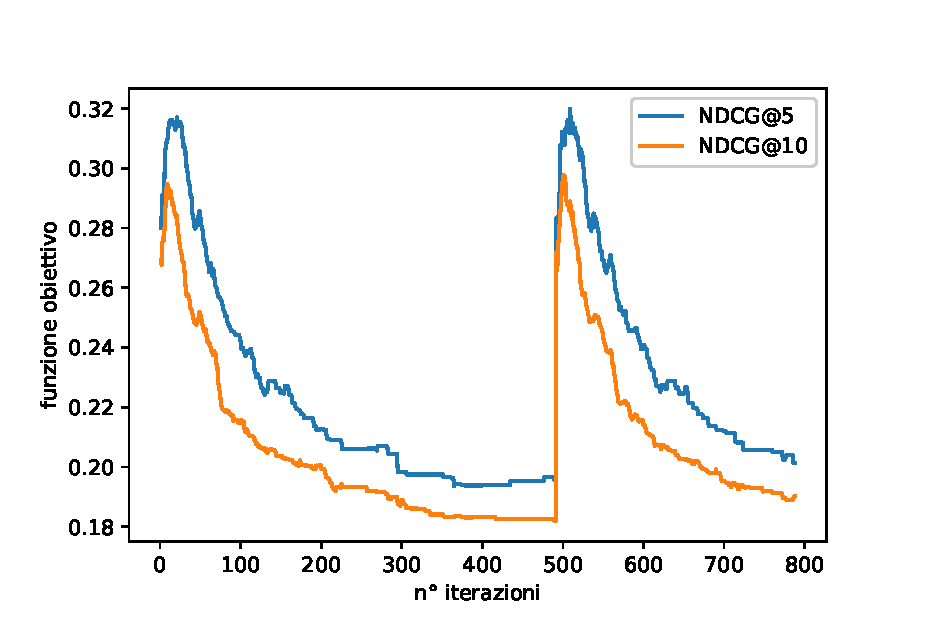
\includegraphics[width=0.7\linewidth]{figure/gs_search}
	\caption[Andamento della funzione obiettivo utilizzando GridSearch]{}
	\label{fig:gssearch}
\end{figure}


Grid Search dopo svariate ore di lavoro non è riuscito a produrre risultati soddisfacenti.

\section{Line Search with Random Restart}

\begin{table}[h!]
	\centering
	\begin{tabular}{|c|c|}
		\hline
		recall@100 &  0.1988 \\
		\hline
		recall@200 & 0.2793  \\
		\hline
		NDCG & 0.3814 \\
		\hline
		NDCG@5 & 0.3188 \\
		\hline
		NDCG@10 & 0.2901 \\
		\hline
		\multicolumn{2}{|c|}{
			$w = [1.071, 0.821, 0.821, 0.821, 0.821, 0.821, 1.071, 0.821, 1.0714, 1.071]$ 
		} \\
	\hline
	\end{tabular}
	\caption{Risultati di Line Search with Random Restart}
\end{table}

\section{Increase Search}

\begin{table}[h!]
	\centering
	\begin{tabular}{|c|c|}
		\hline
		recall@100 &  0.1971  \\
		\hline
		recall@200 & 0.2954  \\
		\hline
		NDCG & 0.4119 \\
		\hline
		NDCG@5 & 0.3542 \\
		\hline
		NDCG@10 & 0.3007 \\
		\hline
		\multicolumn{2}{|c|}{$w = [0.1981, 0.1012, 0.07532, 0.075321, 0.15023, 0.12532, 0.12512, 0.103, 0.0521, 0.2534]$} \\
		\hline
	\end{tabular}
	\caption{Risultati di Increase Search}
\end{table}

\section{Risultati}

Com'è possibile notare il vettore dei pesi migliore è quello che è stato trovato
dall'algoritmo Increase Search, producendo un incremento del $7\%$  rispetto all'orginale BM25.
Pertanto tale algoritmo, avendo a disposizione di un budget di tempo $\mathcal{B}$ nell'ordine
delle ore, performa maggiormente rispetto agli altri.
Ovviamente aumentando $\mathcal{B}$ diventa possibile utilizzare anche gli altri
tipi di algoritmi, quali Grid Search o Line Search with Random Restart.

\section{Test di significatività statistico}

Prima di poter concludere che BM25P con il $w$ ottimo è migliore di BM25, è necessario
fare un test statistico, il cui obiettivo è quello di capire se $\text{BM25P}_w$ $\equiv$ BM25
cioè se essi sono uguali.

Il test è chiamato test di significatività statistico, il quale obiettivo
è quello di capire se due medie provengono da distribuzioni diverse oppure no.
Inannzitutto si deve formulare la \textit{null-hypothesis}, cioè l'ipotesi
della quale vogliamo provarne la falsità.

\begin{esempio}
	Si lancia un dado 10 volte e si calcola la media $\bar{X}_2$. Dopo un giorno si ripete l'esperimento
	e si ricalcola la media $\bar{X}_2$. Molto probabilmente si noterà che $\bar{X}_1 \neq \bar{X}_2$,
	ma tali valori provengono da distrubuzioni diverse?
	Ovviamente no, poiché i dadi sono gli stessi, dunque se la null-hypothesis fosse
	stata $X_1 \equiv X_2$, allora avremmo potuto renderla vera.
\end{esempio}

Dunque in questo caso siamo in grado accetare l'ipotesi perché
sapevamo già a priori che le due distribuzioni erano uguali, ma nel caso
in cui non lo sapessimo?
Uno dei modi più veloci di giudicare la null-hypothesis è quello di eseguire un test statistico.
Accordandoci con l'articolo\cite{10.1145/1321440.1321528}, il miglior test per valutare
due ranker è quello chiamato \textit{Fisher's Randomization Test}.

\subsection{Il test Randomizzato di Fisher}
Tale test si basa sull'ipotizzare che due ranker $\mathcal{R}_1 $ e $\mathcal{R}_2$ siano identici
e che un altro ranker $\mathcal{R}_F$ si impossessi dei risultati di entrambi e
ritorni casualmente o quello di uno o quello di un altro.
Il ruolo giocato da $\mathcal{R}_F$ è di fondamentale importanza, poiché esso produce un risultato
casuale tra i due, pertanto, se essi fossero identici la distrubuzione non cambierebbe.
Ma l'obiettivo principale è quello di calcolare la probabilità che la differenza
di performance tra i due è soltanto dovuta al fatto che $\mathcal{R}_3$ sceglie casualmente
il risultato tra i due ranker.

Per eseguire il test ipotizziamo di avere a disposizione un dataset formato da una lista
di coppie $\langle e_{A}, e_{B}\rangle$, dove la lettera $e$ indica la funzione di valutazione
scelta: nel caso in questione NDCG@5. I pedici $A$ e $B$ indicano invece rispettivamente i due
ranker, dove per semplicità di trattazione abbiamo posto che $A$ è BM25P e $B$ è BM25. Tali valutazioni sono calcolate solo e soltanto su una query,
pertanto abbiamo a disposizione 50 coppie.

\paragraph{Definizioni}
Definiamo le seguenti quantità:

\begin{itemize}
	\item $N$ la lunghezza della lista del dataset (nel caso in questione $N=50$)
	\item $\sigma_A = \sum_{i=1}^{N} e_{A_i}$ e $\sigma_B = \sum_{i=1}^{N} e_{B_i}$
	\item $\bar{e}_A = \frac{\sigma_{A} }{N}$ e  $\bar{e}_B = \frac{\sigma_{B} }{N}$, cioè le relative medie aritmetiche
	\item $d = \sigma_{A} - \sigma_{B}$, cioè la differenza di performance tra i due ranker
\end{itemize}


\begin{algorithm}[h!]
	\SetAlgorithmName{Algoritmo}{}
	\small
	\DontPrintSemicolon
	\SetKwInOut{Input}{Input}
	\SetKwInOut{Output}{Output}
	\Input{$e_A$ lista delle valutazioni del ranker A}
	\Input{$e_B$ lista delle valutazioni del ranker B}
	\Input{$d$}
	\Input{$k$}
	\Input{$\sigma_A, \sigma_B$}
	\Input{$\bar{e}_A, \bar{e}_B$}
	\Output{$p_1,p_2$}
	\BlankLine
	$p_1 = 0, p_2 = 0$\;
	\BlankLine
	\For{$i=1$ \textbf{to} $k$}{
		$a,b = \text{randomChoice}(e_A, e_B)$\;
		$\bar{a} = avg(a)$\;
		$\bar{b} = avg(b)$\;
		
		\BlankLine
		$\delta = \bar{a} - \bar{b}$\;
		\If{$\delta \geq d$}{
			$p_1 = p_1 + 1$\;
		}
		\If{$\left|\delta\right| \geq \left|d\right|$}{
			$p_2 = p_2 + 1$\;
		}
	}
	
	\Return{$\frac{p_1}{k}, \frac{p_2}{k}$}
	\label{alg:spectest}
	\caption{Algoritmo per l'esecuzione del test di randomizzazione di Fisher}
\end{algorithm}

A questo punto si procede scegliendo un numero massimo $k$ di permutazioni
da eseguire, poichè  senza limitazioni  il test avrebbe complessità $\mathcal{O}(2^N)$
e dunque per valori di $N$ elevati ci vorrebbe troppo tempo per eseguirlo.
\\
\\
Successivamente l'algoritmo esegue un ciclo, scorrendo un indice fino ad arrivare a $k$.
Nel corpo del ciclo, essoo prende a caso un elemento della lista di $e_A$ o di $e_B$ e
calcola la differenza di qualità ottenuta.
A seconda dei risultati vengono incrementi i valori $p_1$ o $p_2$, che costituiscono
l'output dell'algoritmo stesso.

Riassumendo, ciò che $\mathcal{R}_3$ esegue è un assegnamento casuale di etichette e
possiamo considerare Il test valido se la scelta è casuale (anche se in questo caso
dobbiamo accontentarci della pseudocasualità).

\paragraph{Il risultato del test}
I valori calcolati dall'algoritmo, cioè $p_1$ e $p_2$, sono due rapporti:

\begin{itemize}
	\item $p_1$ è detto anche ``one-sided-p-value", ovvero il rapporto tra il numero di volte che la differenza
	della valutazione è più grande di quella ipotizzata e il numero di permutazioni
	\item $p_2$ è detto invece ``two-sided-p-value", overo il solito significato di $p_1$ ma utilizzando
	come metrica di differenza il valore assoluto.
\end{itemize}


Per poter valutare dunque la veridicità della \textit{null-hypothesis} si usano tali valori,
cioè $p_1$ e $p_2$ costituiscono un'approssimazione della probabilità che che i due ranker
siano uguali. Solitamente si sceglie un valore $\alpha < 0.05$ per cui si valuta che
se $p_1$ e $p_2$ sono maggiori di $\alpha$ allora l'ipotesi non può essere rifiutata,
mentre se sono minori l'ipotesi è falsa, e dunque i due ranker sono diversi.


\subsection{Esecuzione nel caso di BM25P}
L'esperimento è stato condotto sul solito dataset, isolando le query tal topic file e calcolando la NDCG
per ogni ogni query, sia con BM25P che con BM25P.

Il test ha riportato i seguenti valori

\begin{table}[h!]
	\centering
	\begin{tabular}{|c|c|c|}
		\hline
		\textbf{Misura} & $p_1$ & $p_2$ \\
		\hline
		NDCG  & 0.13218 & 0.26347 \\
		\hline
		NDCG@5 & 0.00082 & 0.00145 \\
		\hline
		NDCG@10 & 0.03454 & 0.06835 \\
		\hline
	\end{tabular}
	\caption{Risultati del test statistico su BM25P}
\end{table}

Considerando i valori standard di $\alpha$, la \textit{null-hypothesis} (BM25P $\equiv$ BM25) può essere considerata falsa.
Questo perché, dato che l'ottimizzazione di BM25P è stata basata sui tagli più piccoli, il test di significatività statistico su NDCG@5 e NDCG@10 
deve avere più peso rispetto a NDCG senza tagli.
Questo risultato inoltre ci mostra che i due ranker, su tagli più grandi, potrebbero essere simili, in quanto $p_2 > p_1 > \alpha$. \footnote{Potrei aggiungere all'appendice anche lo snippet in python?}


\chapter{Risultati sperimentali}

\appendix

\chapter{Codice Java}

\section{Implementazione di BM25P}

\lstinputlisting{code/BM25P.java}

\section{Implementazione di Grid Search}

\lstinputlisting{code/GridSearch.java}

\section{Implementazione di Increase Search}

\lstinputlisting{code/IncreaseSearch.java}

\section{Implementazione del test di Fisher}

Questa parte di codice è stata realizzata prendendo come spunto
l'idea posta da \textit{RankEval}, il cui articolo \cite{rankeval-sigir17} illustra
un modo per eseguire in python il test di randomizzazione
di Fisher.

\lstinputlisting{code/fisher.py}

\clearpage

\bibliographystyle{plain}
\bibliography{mybib}

% \printindex

\chapter*{Ringraziamenti}

Vorrei ringraziare tutte le persone che in qualsiasi modo mi hanno aiutato
ad affrontare questo percorso universitario.
\\
\\
Alla mia famiglia, che ha sostenuto la spesa economica dell'università.
\\
\\
A Eleonora, che nei momenti più difficili e bui si è resa la mia lanterna.
\\
\\
Ai miei professori, che sono stati fonte di ispirazione per ogni
problema.
\\
\\
Agli ingegneri Franco Maria Nardini, Nicola Tonellotto e la dottoressa
Cristina Muntean, che mi hanno guidato pazientemente nell'esperienza
del tirocinio.



\end{document}